\setmodule{10}

%BEGIN_FOLD % ====>>_____ Занятие 1 _____<<====
\begin{class}[number=1]
	\begin{listofex}
		\item Банка краски стоила \( 270 \) рублей. После подорожания она стала стоить на \( 20\% \) дороже. Сколько заплатит покупатель за \( 6 \) банок по новой цене?
		\item На клетчатой бумаге с клетками \( 1*1 \) см изображен треугольник. Найти его площадь квадратных сантиметрах.
		\begin{center}
			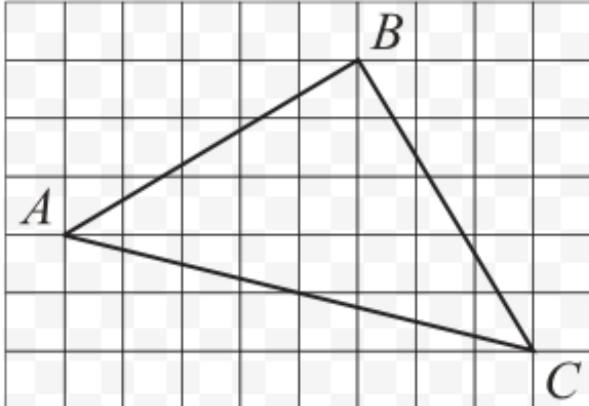
\includegraphics[align=t, width=0.5\linewidth]{../\picpath/MoisenkoL1}
		\end{center}
		\item Упростите выражение: \( \log_414-\log_47 \)
		\item Найдите значение выражения: \( 3\tg33\degree\cdot2\tg57\degree \)
		\item Решите уравнение: \( \sqrt{x^2-x-3}=3 \)
		\item Найдите корень уравнения. В случае, если их несколько, найдите их сумму: \( \log_2(x^2-3x+3)=0 \)
		\item Найдите значение выражения \( \tg\alpha-2\sin\alpha \), если \( \cos\alpha=0,8 \) и \\ \( \dfrac{3\pi}{2}\le\alpha\le2\pi \)
		\item Вычислите значение выражения: \( 2(\sqrt{x}-2)\cdot(\sqrt{x}+2) \), если \( x=6 \)
		\item Решите неравенство: \( 3^{x+3}<\dfrac{1}{27} \)
		\item Найдите область значения функции \( y=\sqrt{\dfrac{x+2}{2x-8}} \)
		\item В таксомоторной фирме \( 40 \) машин: \( 13 \) желтых, \( 12 \) черных. Остальные --- белые. Определить вероятность, что прибывшая по заказу машина не черная.
		\item Найдите точку минимума функции: \( y=x^3-18x+6 \)
		\item Найдите объём \( V \) конуса, образующая которого равна \( 3 \) и наклонена к плоскости основания под углом \( 30\degree \). В ответ укажите \( \dfrac{V}{\pi} \).
		\item Дана правильная четырёхугольная пирамида. Сторона основания равна \( 6 \). Высота равна \( 4 \). Найдите синус угла наклона бокового ребра к основанию пирамиды.
		\item Решите уравнение \( \cos\left( \dfrac{\pi}{4}-10x \right)=0 \)
		\item В правильной треугольной призме со стороной основания \( 6 \) и высотой \( 4 \) проведено сечение через сторону нижнего основания и противоположную вершину верхнего основания.
		Определить площадь сечения.
		\item Решите систему неравенств:
		\( \begin{cases} \dfrac{9^x-1}{3-3^x}<0 \\ \log_2(x+2)\le1 \end{cases} \)
	\end{listofex}
\end{class}
%END_FOLD

%BEGIN_FOLD % ====>>_____ Занятие 2 _____<<====
\begin{class}[number=2]
	\begin{listofex}
		\item .
	\end{listofex}
\end{class}
%END_FOLD

%BEGIN_FOLD % ====>>_ Домашняя работа 1 _<<====
\begin{homework}[number=1]
	\begin{listofex}
		\item Домашняя работа 1
	\end{listofex}
\end{homework}
%END_FOLD

%BEGIN_FOLD % ====>>_____ Занятие 3 _____<<====
\begin{class}[number=3]
	\begin{listofex}
		\item ю
	\end{listofex}
\end{class}
%END_FOLD

%BEGIN_FOLD % ====>>_____ Занятие 4 _____<<====
\begin{class}[number=4]
	\begin{listofex}
		\item Занятие 4
	\end{listofex}
\end{class}
%END_FOLD

%BEGIN_FOLD % ====>>_ Домашняя работа 2 _<<====
\begin{homework}[number=2]
	\begin{listofex}
		\item Домашняя работа 2
	\end{listofex}
\end{homework}
%END_FOLD

%BEGIN_FOLD % ====>>_____ Занятие 5 _____<<====
\begin{class}[number=5]
	\begin{listofex}
		\item Занятие 5
	\end{listofex}
\end{class}
%END_FOLD

%BEGIN_FOLD % ====>>_____ Занятие 6 _____<<====
\begin{class}[number=6]
	\begin{listofex}
		\item Занятие 6
	\end{listofex}
\end{class}
%END_FOLD

%BEGIN_FOLD % ====>>_ Домашняя работа 3 _<<====
\begin{homework}[number=3]
	\begin{listofex}
		\item Домашняя работа 3
	\end{listofex}
\end{homework}
%END_FOLD

%BEGIN_FOLD % ====>>_____ Занятие 7 _____<<====
\begin{class}[number=7]
	\title{Подготовка к проверочной}
	\begin{listofex}
		\item Занятие 7
	\end{listofex}
\end{class}
%END_FOLD

%BEGIN_FOLD % ====>>_ Проверочная работа _<<====
\begin{exam}
	\begin{listofex}
		\item Проверочная
	\end{listofex}
\end{exam}
%END_FOLD